% document's head

\phantom{42}
\vspace{20mm}

\begin{center}
    \LARGE \textsc{Лабораторная работа} \\
    \vspace{3 mm}
    \large Измерение частоты темнового счёта и шум-фактора твердотельного фотоумножителя SiPM
\end{center}

% \hrule

\phantom{42}

\begin{flushright}
    \begin{tabular}{rr}
    % written by:
        % \textbf{Источник}: 
        % & \href{__ссылка__}{__название__} \\
        % & \\
        % \textbf{Лектор}: 
        % & _ФИО_ \\
        % & \\
        \textbf{Автор работы}: 
        & Хоружий Кирилл \\ 
        & Кузнецова Арина \\
        & Евгений Дедков \\
        & Александр Двуреченский \\
        & Яушев Михаил  \\ 
        & \\
    % date:
        \textbf{От}: &
        \textit{\today}\\
    \end{tabular}
\end{flushright}

\thispagestyle{empty}

\vspace{10mm}


\subsection*{Цель работы}
\begin{enumerate*}
    \item Измерение ВАХ лавинного фотодиода с отрицательной обратной сязью.
    \item Определение емкости ячейки $C$ и пробойного напряжения $\sub{U}{br}$ лавинного фотодиода.
\end{enumerate*}


\subsection*{Оборудование}
Источник-измеритель Keithley 236 (1), 
лавинный фотодиод SiPM (2), 
светоизолированный бокс (3) со светодиодом (4), поключенный к реугулируемому источнику напряжения (5).

% \subsection*{Рабочая установка}

\begin{figure}[h]
    \centering
    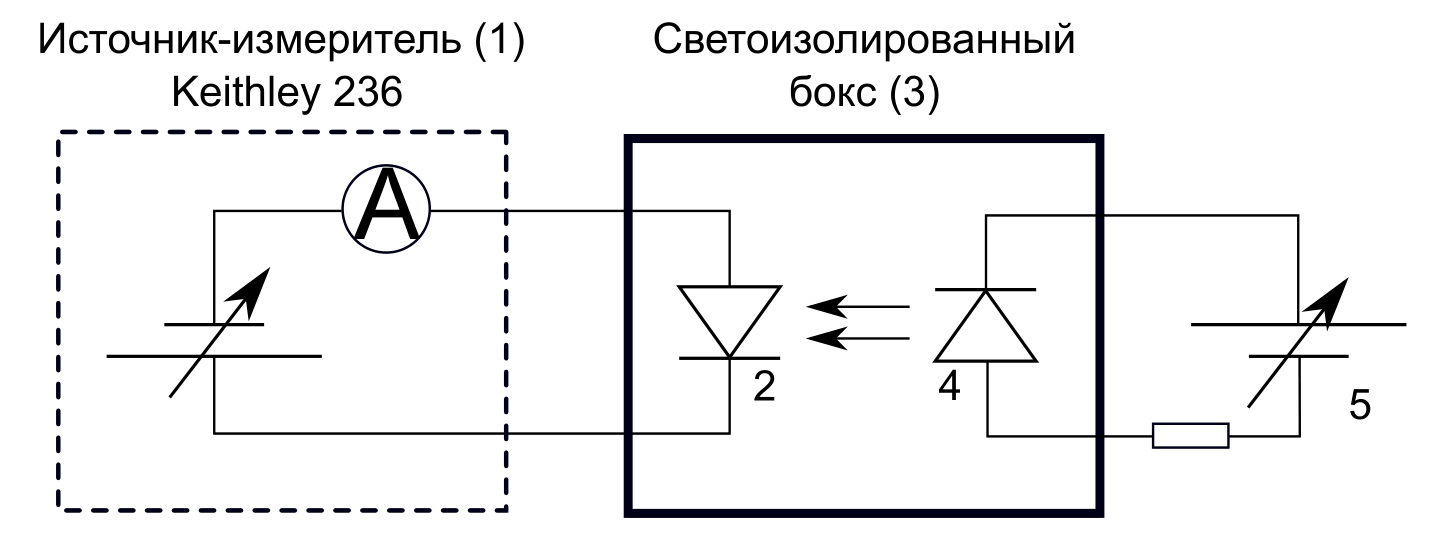
\includegraphics[width=0.5\textwidth]{figures/exp.png}
    \caption{Схема установки для измерения световых и темновх вольт-амперных характеристик фотодиода}
    \label{fig:01}
\end{figure}





\newpage
